\documentclass[12pt]{article}

% Packages
\usepackage{lipsum}
\usepackage{setspace}
\usepackage{indentfirst}
\usepackage{geometry}
\usepackage[nonumberlist, toc]{glossaries}
\usepackage{graphicx}
\usepackage{caption}
\usepackage{subcaption}
\usepackage{tabularx}
\usepackage{booktabs}
\usepackage[numbered]{./latex/mcode}
\usepackage{enumitem}
\usepackage{xcolor}
\usepackage [autostyle, english = american]{csquotes}
\usepackage{fancyhdr}
\usepackage{amsmath}

% Formatting
\geometry{letterpaper, portrait, margin=.85in}

\pagestyle{fancy}
\lhead{MSXII Suspension Parameters}
\rhead{Midnight Sun Solar Car Team}

\MakeOuterQuote{"}

\begin{document}

% Title Ppage
\begin{titlepage}
	\vspace*{3cm}
	\centering
	
\includegraphics[width=.2\textwidth]{./LaTex/midnightSunLogoCircle.png}\par
	\vspace{1.5cm}
	{\scshape\LARGE Midnight Sun Solar Car Team \par}
	{\scshape\large University of Waterloo\par}
	\vspace{1.5cm}
	{\huge\bfseries MSXII Suspension Parameters\par}
	\vspace{0.2cm}
	\large Prepared for Project 3 of ME321 Winter 2017
	\vfill
	Prepared by:\par
	Devon Copeland\par
	\vspace{1cm}
	\today\par
\end{titlepage}

% Main Matter
\section{Background}
\subsection{Vehicle Design}
Midnight Sun Twelve (MSXII) is a cruiser class solar electric vehicle being designed with the goal of competing in the 2018 American Solar Challenge (ASC 2018) and the 2019 World Solar Challenge (WSC 2019). Cruiser class vehicles are must be multi-occupant and are designed with the intent of being more practical than a typical solar car. Because of the unique requirements of this class, the spring rates and target damping coefficients on MSXII's suspension must be selected to optimize for efficient while still keeping driver comfort in mind. This report proposes and analytical technique for determining the response of the suspension system to a variety of road conditions. 

\subsection{Important Vehicle Parameters}
Table \ref{tab:params} lists predicted vehicle parameters that are of importance to the design and analysis of the suspension. 
\begin{table}[]
	\centering
	\caption{Important Vehicle Parameters}
	\label{tab:params}
	\begin{tabular}{lll}
	Mass                             & 500  & $kg$                    \\
	Distance from Front Wheel to CoG & 1.32 & $m$                     \\
	Moment of Inertia                & 550  & $kgm^2$ \\
	Wheelbase                        & 1.6  & $m$                    
	\end{tabular}
\end{table}
\subsection{Front Suspension} 
MSXII's front suspension comprises of a double wishbone linkage with an outboard coilover. Important dimensions required for subsequent analysis are shown in Figure \ref{fig:}:

\subsection{Rear Suspension} 
MSXII's rear suspension comprises of independent trailing arms allowing for zero scrub and thus less rolling resistance. Dimensions required for subsequent analysis are shown in Figure \ref{fig:}:

\subsection{Selecting Spring Rates}

\section{Suspension Model}

\subsection{Overview}
MSXII's suspension is modelled using a point mass connected to two vertical, linear spring mass damper systems at the two wheels. This half car model assumes infinite tire stiffness and that the vehicle pitches about it's center of gravity. Figure \ref{fig:systemModel} describes the proposed model where: 
\begin{align*}
	\theta & \text{ is the pitch angle about positive x axis}\\        
	x_0 & \text{ is the displacement of the center of gravity in the vertical axis} \\
	x_1 \text{ \& } x_2 & \text{ are the displacements of the mounting points for the front and rear wheels respectively} \\
	y_1 \text{ \& } y_2 & \text{ is the change in road elevation below the front  and rear wheels respectively} \\
	M & \text{ is the mass of the vehicle} \\
	I & \text{ is the moment of inertia normal to the half car plane at the center of gravity} \\
	k1,k2,c1 \text{ \& } c_2 & \text{ are the spring and damping coefficients} \\
	a \text{ \& } b & \text{ are the distances from center of gravity to the front and rear wheels respectively}
\end{align*}
\begin{figure}[h!]
	\centering
	\label{fig:systemModel}
	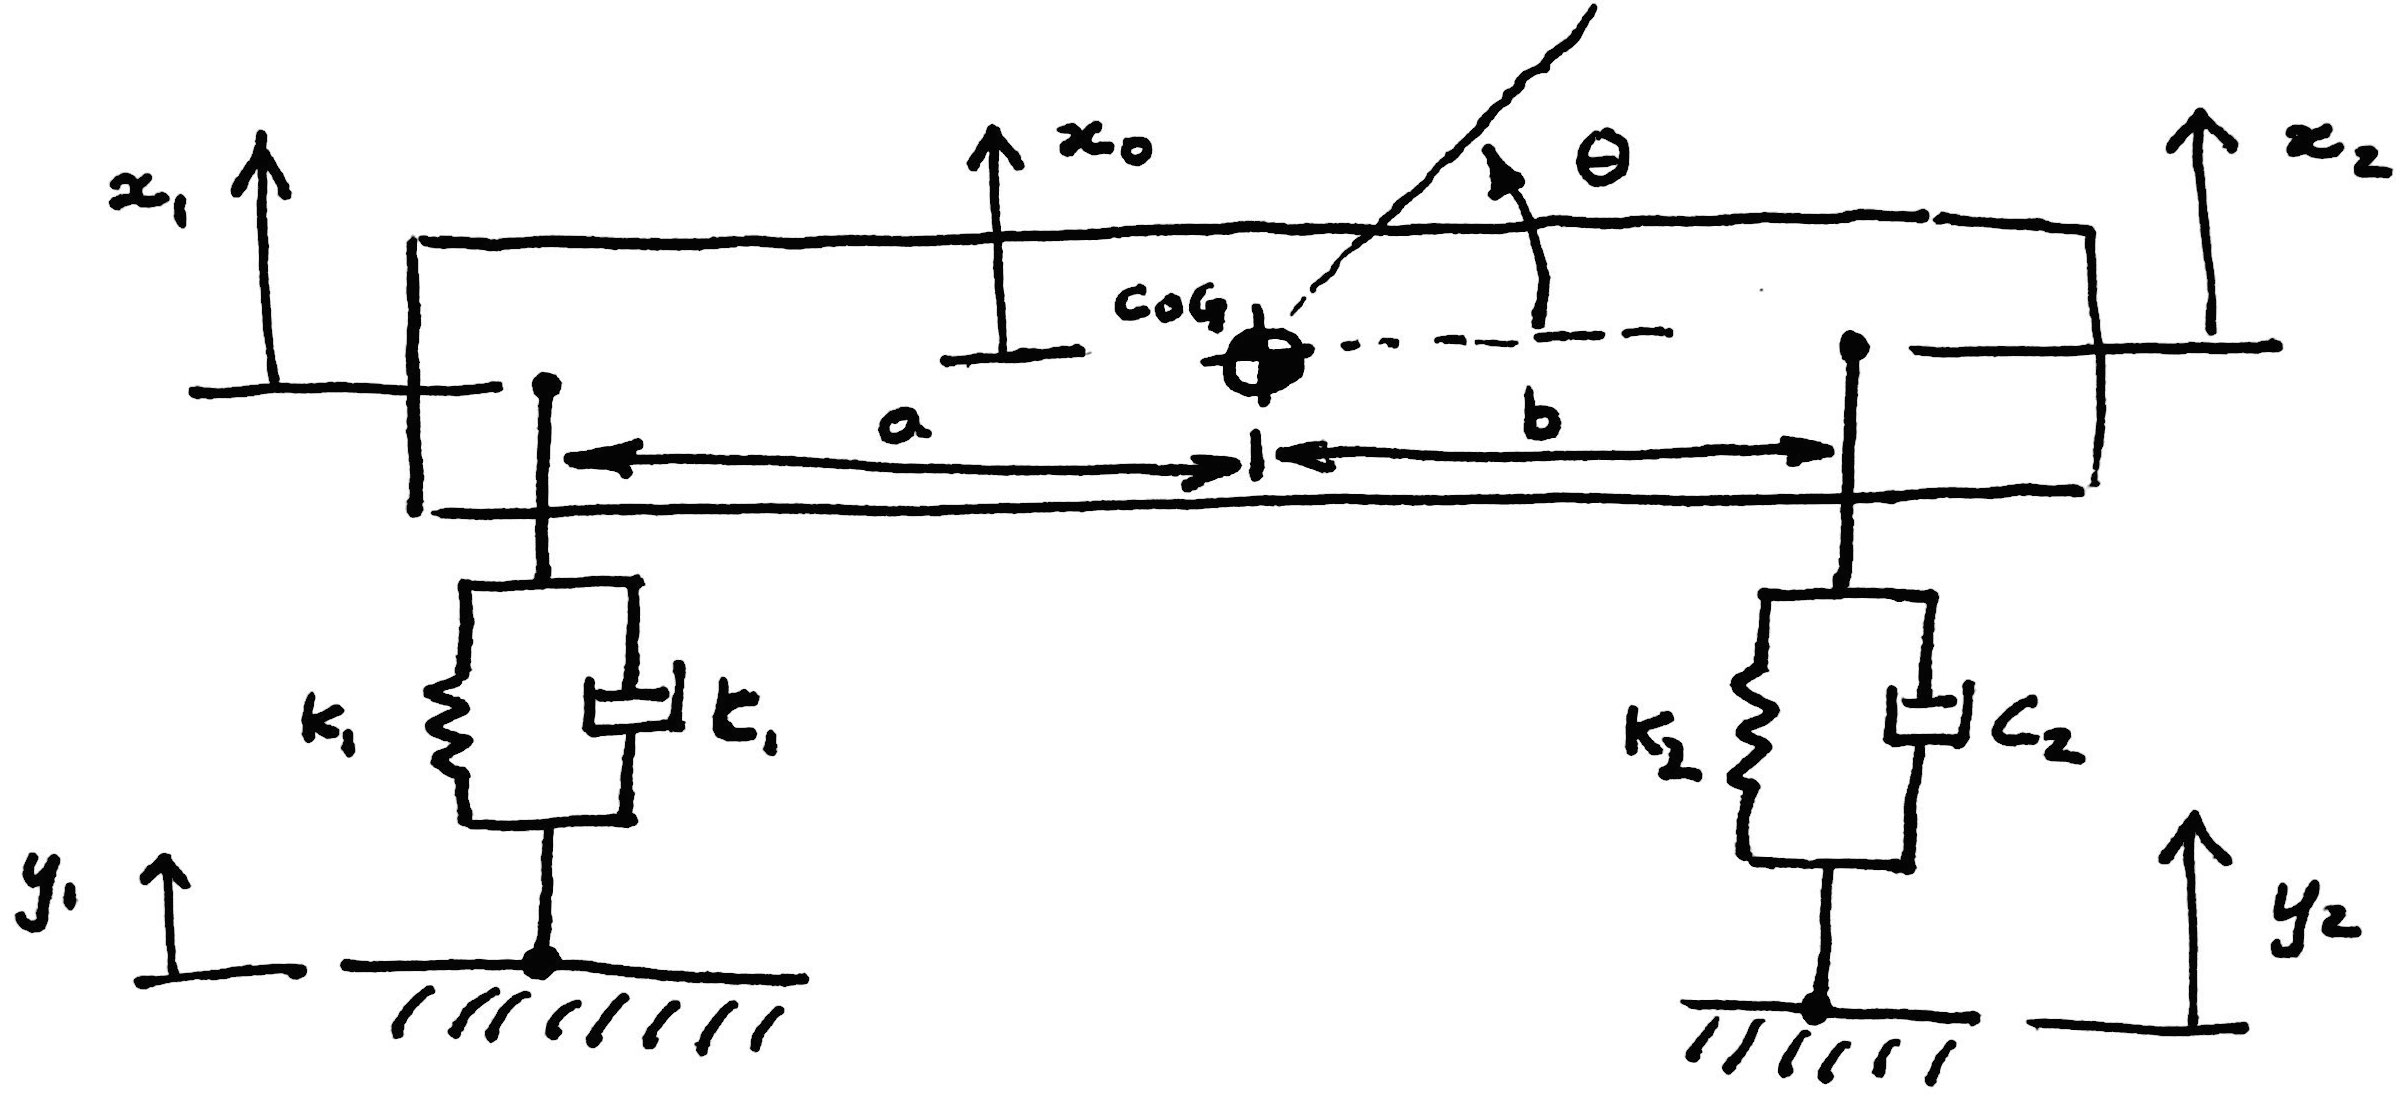
\includegraphics[width=.8\textwidth]{./LaTex/systemModel.jpg}
	\caption{Half car model with infinite tire stiffness}
\end{figure}

\subsection{Equations of Motion}
The spring mass damper system shown in Figure \ref{fig:systemModel} can be described by the folowing two differential equations: 
\begin{equation}
	M \ddot x + c_1(\dot x_1 - \dot y_1) + c_2(\dot x_2 - \dot y_2) + k_1(x_1 - y_1) + k_2(x_2 - y_2) = 0
\end{equation}
\begin{equation}
	I \ddot\theta - ac_1(\dot x_1 - \dot y_1) + bc_2(\dot x_2 - \dot y_2) - ak_1(x_1 - y_1) + bk_2(x_2 - y_2) = 0
\end{equation}
Rearranging to move the inputs $y_1$ and $y_2$ to right hand side: 
\begin{equation}
	M \ddot x + c_1\dot x_1 + c_2\dot x_2 + k_1x_1 + k_2x_2 = c_1\dot y_1 + c_2\dot y_2 + k_1y_1 + k_2y_2
\end{equation}
\begin{equation}
	I \ddot\theta - ac_1\dot x_1 + bc_2\dot x_2 - ak_1x_1 + bk_2x_2 = -ac_1\dot y_1 + bc_2\dot y_2 - ak_1y_1 + bk_2y_2
\end{equation}
By assuming small pitch angles, $\theta$, the angle between the spring mass damper system becomes approximately perpendicular and the displacements $x_1$ and $x_2$ can be approximated as follows:
\begin{equation}
	x_1 = x_0 - a\theta
\end{equation}
\begin{equation}
	x_2 = x_0 + b\theta
\end{equation}
It follows that the time derivatives of the above two equations are: 
\begin{equation}
	\dot x_1 = x_0 - a\dot\theta
\end{equation}
\begin{equation}
	\dot x_2 = x_0 + b\dot\theta
\end{equation}
Substituting into the original differential equations: 
\begin{equation}
	M \ddot x + \dot x_0(c_2+c_1) + \dot\theta(bc_2-ac_1) + x_0(k_2+k_1) + \theta(bk_2-ak_1)= c_1\dot y_1 + c_2\dot y_2 + k_1y_1 + k_2y_2
\end{equation}
\begin{equation}
	I \ddot\theta + \dot x_0(bc_2-ac_1) + \dot\theta(b^2c_2-a^2c_1) + x_0(bk_2-ak_1) + \theta(b^2k_2+a^2k_1) = -ac_1\dot y_1 + bc_2\dot y_2 - ak_1y_1 + bk_2y_2
\end{equation}
By taking the unilateral laplace transform of the above two equations with all initial conditions set to zero, the following $s$ domain equations are obtained:
\begin{equation}
	\left[Ms^2+(c_2+c_1)s+(k_2+k_1)\right]X_0 + \left[(bc_2-ac_1)s+(bk_2+ak_1)\right]\Theta = c_1sY_1 + c_2sY_2 + k_1Y_1 + k_2Y_2
\end{equation}
\begin{equation}
	\left[(bc_2-ac_1)s+(bk_2-ak_1)\right]X_0 + \left[Is^2+ (b^2c_2+a^2c_1)s+(b^2k_2+a^2k_1)\right]\Theta = c_1sY_1 + c_2sY_2 + k_1Y_1 + k_2Y_2
\end{equation}
The above two equations can be expressed in matrix form as follows: 
\begin{equation}
	\label{eq:matrix1}
	\begin{bmatrix} 
	Q_{Ax}(s) & Q_{A\Theta}(s) \\
	Q_{Bx}(s) & Q_{B\Theta}(s)
	\end{bmatrix}
	\begin{bmatrix} 
	X_0 \\
	\Theta 
	\end{bmatrix}
	= 
	\begin{bmatrix} 
	P_{A1}(s) \\
	P_{B1}(s)
	\end{bmatrix}Y_1 +
	\begin{bmatrix} 
	P_{A2}(s) \\
	P_{B2}(s)
	\end{bmatrix}
	Y_2
\end{equation}
If it is assumed that the rear tire of the car experiences the exact same road conditions as the front tire, $Y1$ and $Y2$ can be expressed as functions of the same input, $Y$ where $Y2$ is simply a phase shifted version of $Y1$:
\begin{equation}
	\begin{split}
		y_1(t) &= y(t)\\
		y_2(t) &= y(t-t_0)
	\end{split} \implies
	\begin{split}
		Y_1(s) &= Y(s)\\
		Y_2(s) &= Y(s)e^{-st_0}
	\end{split}
\end{equation}
Equation \ref{eq:matrix1} can then be rewritten as follows:
\begin{equation}
	\label{eq:matrix1}
	Q
	\begin{bmatrix} 
	X_0 \\
	\Theta 
	\end{bmatrix}
	= 
	\left(\left[P_1\right]+\left[P_2\right]e^{-st_0}\right)Y
\end{equation}
Since the system is linear linear, the above matrix equation can be solved in two parts to obtain the transfer functions for $X_0$ and $\Theta$:
\begin{equation}
	\frac{\begin{bmatrix} 
		X_0 \\
		\Theta 
	\end{bmatrix}}{Y} =
	\left[H\right] = 
	\left[H_1\right] + \left[H_2\right] = 
	[Q^{-1}][P_1] + [Q^{-1}][P_1]e^{-st_0} 
\end{equation} 

\section{Analysis}
\subsection{Natural Frequency}
Using the MATLAB script show in Appendix \ref{app:code}, the transfer function $H(s)$ is solved for symbolically and the parameters for $I$, $M$, $k_1$, $k_2$, $a$ and $b$ are substituted into the equation while the damping coefficients $c_1$ and $c_2$ are set to zero. The inverse laplace transform is then taken to obtain the impulse response as shown in Figure \ref{fig:impResp}.
\begin{figure}[h!]
	\centering
	\label{fig:impResp}
	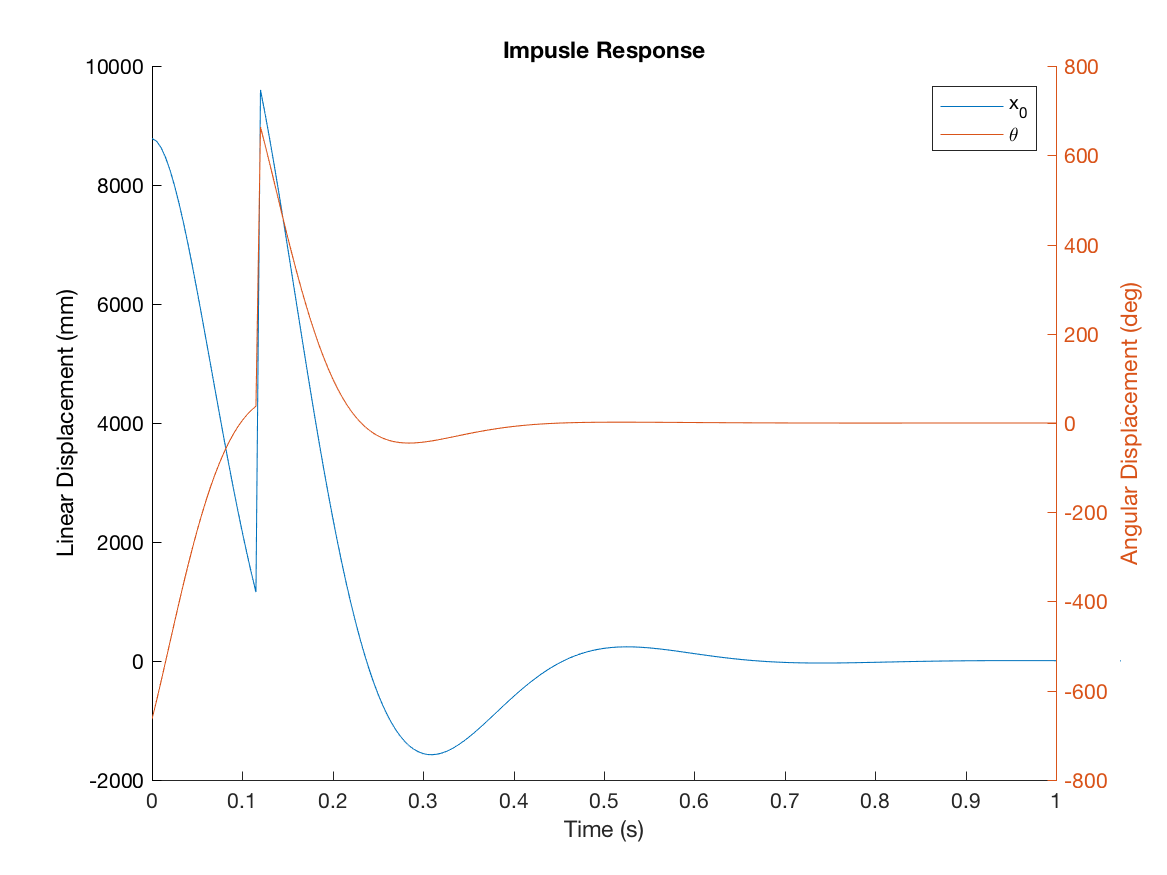
\includegraphics[width=.8\textwidth]{./matlab/impResp.png}
	\caption{Undamped Impulse Response}
\end{figure}

By performing an Fast Fourier Transform on the undamped system the harmonics of the system can be approximated as shown in Figure \ref{fig:fftImpResp}. A sampling frequency of 200Hz and and a window of 30s was used for the FFT.
From figure \ref{fig:fftImpResp}, the largest harmonics of the system occur at Hz for translational displacement and Hz for angular displacement. 
\begin{figure}[h!]
	\centering
	\label{fig:impResp}
	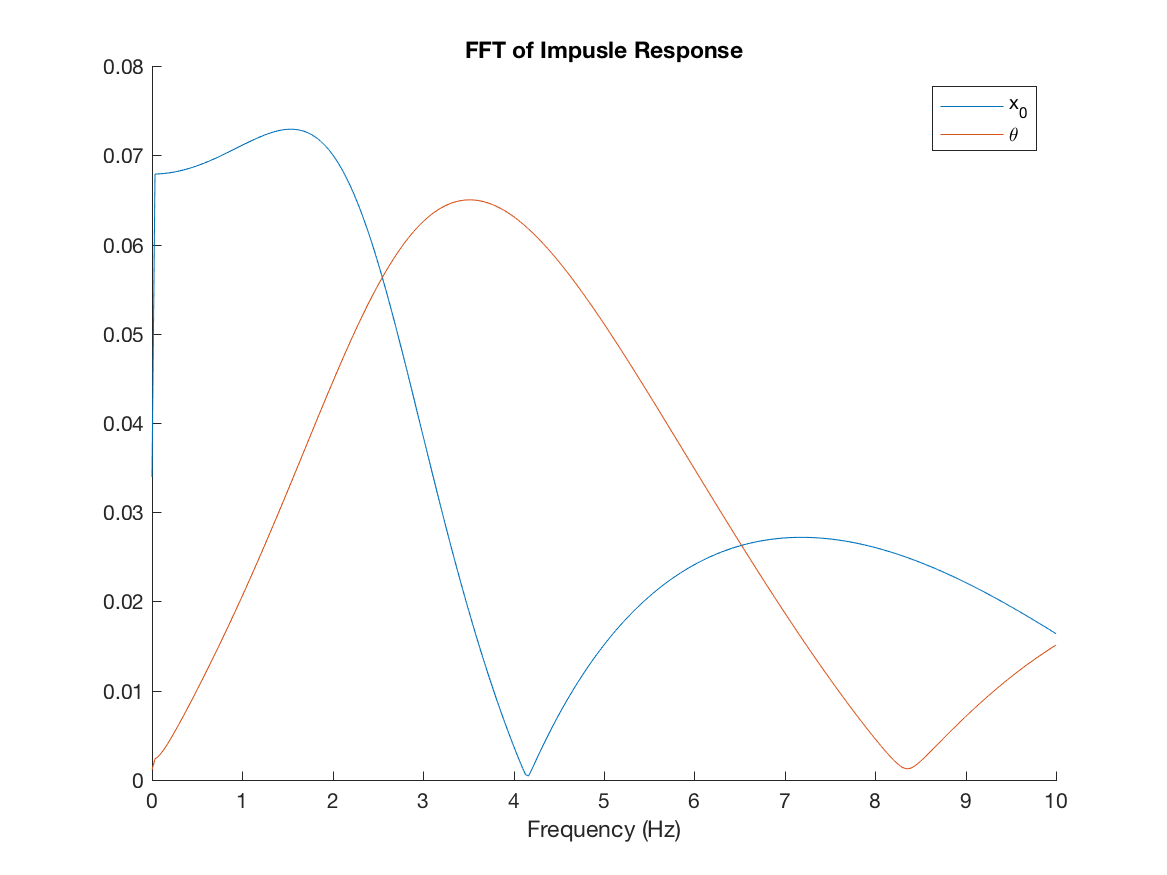
\includegraphics[width=.8\textwidth]{./matlab/fftImpResp.png}
	\caption{FFT of the Undamped Impulse Response}
\end{figure}

\subsection{Critical Damping}


\subsection{Force Response}
\subsection{Worst Case Total Response}

% Appendix
\pagebreak
\appendix
\section{MATLAB Source Code}
\label{app:code}
\lstinputlisting[breaklines=true]{./matlab/createTransferFunctions.m}

\end{document}